Ahora procederemos a analizar, experimentar y discutir los métodos que conciernen al rankeo de páginas Web. Recordemos que en este trabajo se utilizó el modelo PageRank para modelar el rankeo de páginas web utilizando cadenas de Markov y se implementó una versión optimizada especialmente para este problema, presentada en \cite{Kamvar2003}

\subsubsection{Convergencia de PageRank}
Para los experimentos de velocidad de convergencia y rendimiento en general de PageRank utilizamos los datasets de \cite{SNAP}. Para eso, elegimos tres datasets de diferentes tamaños y coeficiente de conectividad \footnote{Con esto nos referimos a que tan conectado está el grafo, esto puede medirse por ejemplo como $\frac{2e}{v(v-1)}$, donde $e$ son las aristas del grafo y $v$ los vertices, dado que el grafo completo tiene $\frac{v(v-1)}{2}$ aristas.}, web-Stanford, web-NotreDame y web-Google.

\begin{figure}[H]
\centering
\begin{tabular}{| c | c | c |}
  \hline
  Dataset & Vértices & Aristas \\ \hline \hline
  web-Stanford & 281.903 & 2.312.497 \\ \hline
  web-NotreDame & 325.729 & 1.497.134 \\ \hline
  web-Google & 916.428 & 5.105.039 \\ \hline
\end{tabular}
\end{figure}


Lo primero que se puede decir de este Datasets es que la diferencia de cantidad de vértices de cada uno nos va a permitir analizar como varía según el tamaño de la red. 

Además, notemos como el dataset web-Stanford está mucho más conectado que el dataset web-NotreDame, dado que tiene menos vértices pero más aristas. Creemos que esto va a impactar negativamente en la performance, dado que sobre una red poco conectada el algoritmo va a converger más rápido.

Eso se puede notar fácilmente si se piensa en el grafo que es totalmente disconexo. En ese caso, todas las entradas de la matriz van a valer $\frac1n$, y el método de la potencia va a converger en un paso.

Otra cosa que podemos pronosticar (en parte porque en \cite{Kamvar2003} pasa eso) es que entre más cercano sea $c$ a 1 (es decir, el navegante aleatorio se teletransporta menos), más lento va a converger.

Al igual que antes, para entender intuitivamente que está pasando, podemos analizar el caso extremo $c = 0$. En este caso, la probabilidad de que el navegante se teletransporte es siempre 1, por lo que volvemos al caso anterior en el que todos los coeficientes de la matriz van a valer $\frac1n$, por lo que se convergerá en un paso.

Concluidas las hipótesis relacionados a la convergencia del método, procedamos a ver los resultados de los experimentos.


\begin{figure}[H]
\centering
\begin{minipage}{0.48\textwidth}
  \centering
    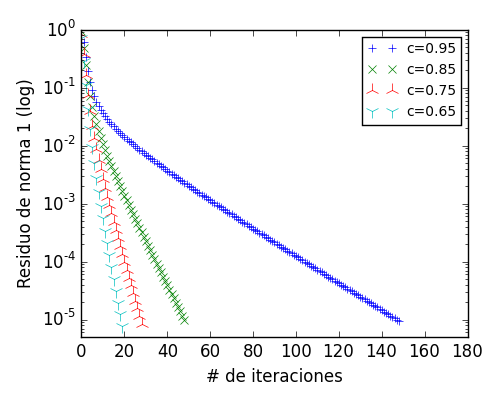
\includegraphics[width=1\textwidth]{imgs/convergencia-stanford.png}
  \caption{\footnotesize{Comparación de la velocidad de convergencia del el método para el dataset web-Stanford.}}
  \label{fig:conv1}
\end{minipage}
\hspace{0.02\textwidth}
\begin{minipage}{0.48\textwidth}
  \centering
    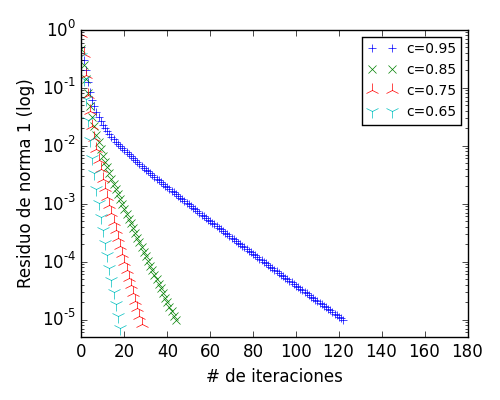
\includegraphics[width=1\textwidth]{imgs/convergencia-notredame.png}
  \caption{\footnotesize{Comparación de la velocidad de convergencia del el método para el dataset web-NotreDame.}}
  \label{fig:conv2}
\end{minipage}
\begin{minipage}{0.5\textwidth}
  \centering
    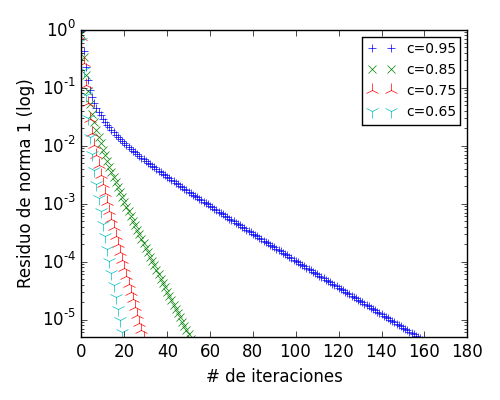
\includegraphics[width=1\textwidth]{imgs/convergencia-google.png}
  \caption{\footnotesize{Comparación de la velocidad de convergencia del el método para el dataset web-Google.}}
  \label{fig:conv3}
\end{minipage}
\end{figure}


Primero notemos algo más o menos sorprendente: la cantidad de iteraciones requeridas por el método no varía demasiado, sobre todo para valores chicos de $c$. Creemos que esto se debe a propiedades generales del método de la potencia, que sin embargo son díficiles de analizar y están fuera del alcance de este trabajo.

Se puede notar además que para los valores más pequeños de $c$ la cantidad de iteraciones correspondientes a cada dataset es prácticamente igual.

Una cosa importante para decir, de la cual vamos a hablar en profundidad más adelante, es que aunque la cantidad de iteraciones sea parecida, el costo de cada iteración es mayor a más grande es la matriz y a más valores no nulos tiene, por lo que las figuras \ref{fig:conv1}, \ref{fig:conv2} y \ref{fig:conv3} no deben intepretarse como el tiempo que requiere el algoritmo para correr.

Sin embargo, una cosa interesante a analizar es qué $c$ usar. Como vimos, usar un $c$ pequeño disminuye el tiempo de cómputo requerido. Sin embargo, disminuir el $c$ también puede impactar en el resultado. Dado que el factor de teletransportación $1-c$ es más alto, de alguna manera el resultado es menos significativo, debido a que se hace más uniforme, como explicamos antes. 
En \cite{Chakrabarti}, por ejemplo, se sugiere que $c$ debería ser elegido basado en la conectividad del grafo.


Otro experimento muy interesante que realizamos es cambiar el criterio de parada del algoritmo iterativo. En particular, lo que hicimos fue cambiar la norma con la que medimos la diferencia entre dos vectores de sucesivas iteraciones. Para ello utilizamos las normas $||-||_1$, $||-||_2$ y $||-||_{\infty}$.

\begin{figure}[H]
\centering

    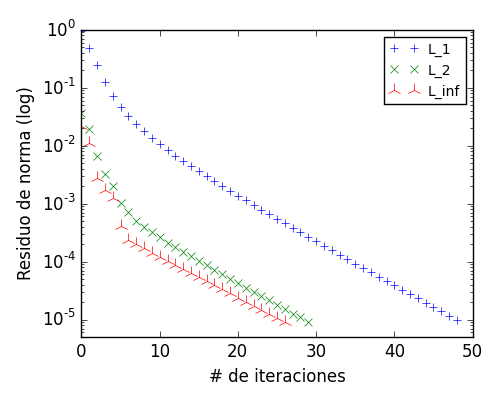
\includegraphics[width=0.6\textwidth]{imgs/convergencia-norma.png}
  \caption{\footnotesize{Comparación de la velocidad de convergencia del el método para el dataset web-Stanford, variando la norma del criterio de parada.}}
  \label{fig:conv-norma}
\end{figure}

Como se observa en la figura \ref{fig:conv-norma}, cuando se utiliza la norma 1 para el criterio de parada, se requieren más iteraciones para terminar. Esto se debe a que la norma 1 es la más \emph{exigente}. 

Se puede probar fácilmente que para todo vector $x$, $||x||_1 \geq ||x||_2 \geq ||x||_{\infty}$ y esto explica claramente los resultados del experimento.



\subsubsection{Rendimiento de PageRank}
A continuación analizaremos el rendimiento del algoritmo de PageRank implementado en este trabajo, es decir, el de \cite{Kamvar2003}. Para ello, utilizaremos los mismos datasets que en la sección anterior.

\begin{figure}[H]
\centering
\begin{tabular}{| c | c | c | c |}
  \hline
  Dataset & Vértices & Aristas & Tiempo (segundos) \\ \hline \hline
  web-Stanford & 281.903 & 2.312.497 & 7.81882 \\ \hline
  web-NotreDame & 325.729 & 1.497.134 & 3.38163 \\ \hline
  web-Google & 916.428 & 5.105.039 & 23.7367 \\ \hline
\end{tabular}

  \caption{\footnotesize{Comparación de los tiempos que requiere el algoritmo para distintos datasets. Fue ejecutado con $c = 0.85$ y $tolerancia = 0.00001$.  Se tomó el promedio de 20 mediciones.}}
  \label{fig:tiempos1}
\end{figure}

Podríamos empezar a sacar conclusiones apresuradas sobre estos datos, pero para que sean más significativos, preferimos realizar otro experimento antes de comenzar el análisis.
Este experimento consiste en dividir el algoritmo en 2: primero el armado de la matriz (recordemos que como representamos la matriz en CRS este no es un paso trivial) y luego el paso de método de la potencia optimizado presentado en \cite{Kamvar2003}.

Esto nos permitirá ver mejor el problema y tener datos más detallados, con el objetivo de poder analizar mejor que es lo que sucede.

\begin{figure}[H]
\centering
\begin{tabular}{| c | c | c | c |}
  \hline
  Dataset & Tiempo total & Armado de matriz & Método de la potencia \\ \hline \hline
  web-Stanford & 7.81882 & 1.8968 & 5.91098 \\ \hline
  web-NotreDame &  3.38163 & 0.978923 & 2.42743 \\ \hline
  web-Google & 23.7367 & 4.30584 & 18.9483 \\ \hline
\end{tabular}

  \caption{\footnotesize{Comparación de los tiempos que requiere el algoritmo para distintos datasets. Fue ejecutado con $c = 0.85$ y $tolerancia = 0.00001$. Se tomó el promedio de 20 mediciones. Todos los tiempos son en segundos. Las sumas probablemente no den bien porque fueron tomadas en diferentes mediciones. }}
  \label{fig:tiempos2}
\end{figure}


Ahora, teniendo toda la información que nos proveen la figura \ref{fig:tiempos1}, \ref{fig:tiempos2} y los experimentos de la sección anterior, podemos hacer un análisis completo y riguroso.

Podemos concluir primero que el paso más costoso del algoritmo es el método de la potencia. Justamente por eso \cite{Kamvar2003} se ocupa de intentar optimizar ese paso, dado que optimizarlo va a impactar fuertemente en el rendimiento general de la aplicación.


Otro aspecto interesante para ver es, como aunque las iteraciones requeridas para cada dataset son bastante similares, el costo de cada operación es muy distinto, pues el tamaño de los vectores varía, y las entradas no nulas de la matriz son distintas. 

De hecho, este experimento nos permite confirmar que el paso más costoso es realizar el producto de la matriz y el vector $P^t x^{(k)}$, ya que se puede ver como el método de la potencia en el caso de web-NotreDame tarda menos que en el caso de web-Stanford, aunque los vectores sean más largos. 

Esto se debe a que la matriz de web-NotreDame es más esparsa, y al multiplicar $Ax$ con $A$ representada en CRS, el costo resulta lineal en la cantidad de elementos no nulos de la matriz. Esta última está intimamente relacionada con la cantidad de aristas del grafo. De esta manera se explica fácilmente el comportamiento a priori extraño de el algoritmo sobre estos datasets.


